\subsubsection{Encrypt and decrypt}
The encrypted payload $\delta$ is where the actual message is hidden. This is computed in different layers using a wide block cipher encryption algorithm and is decrypted at each stage of mixing which is basically a pseudo-random permutation process (PRP). $\delta$ is repeatedly encrypted via keys derived from the DH key exchange between the packet’s group element $\alpha_i$ and the public key of each node in the path $y_i$.

\paragraph{Notation}
Let $j$ be the block size in bits, which will typically be large. Let $H_u$ be a keyed hash function with the key $u$ for the payload. $u$ consists of four independent keys, $u_1$, $u_2$, $u_3$, and $u_4$, which $A$ derives from the master keys $\varphi_0$, $\varphi_1$, $\varphi_2$, and $\varphi_3$ using the HKDF key derivation function explained in \lcnameref{sec:proofofrelay} section using the packet tag as hash key. The derivation is as follow:

$$HKDF.expand(h_b, |h_b|,\varphi_0, |\varphi_i + PRP_IV_LENGTH|, hash\_Key\_PRP)$$


\textbf{Expand} This step takes $\varphi_i$, as a seed and creates output key material $u_i$ for all $1\le i < 4 $ which is expanded from hashes of $\varphi_i$ and an optional info message (salt). The process occurs as follows:

Of the four keys, $u_1$ and $u_3$ will be used to key the stream cipher, while $u_2$ and $u_4$ are used to key the hash function. Sphinx uses the LIONESS wide block cipher scheme for encryption and decryption purposes. Let $S_u$ be a pseudorandom function (stream cipher) which given the input $m$ will generate an output of arbitrary length. We add a padding tag $\tau$ to $m$ before encryption and a 0-padding string as follows:

\begin{figure}[H]
    \centering
    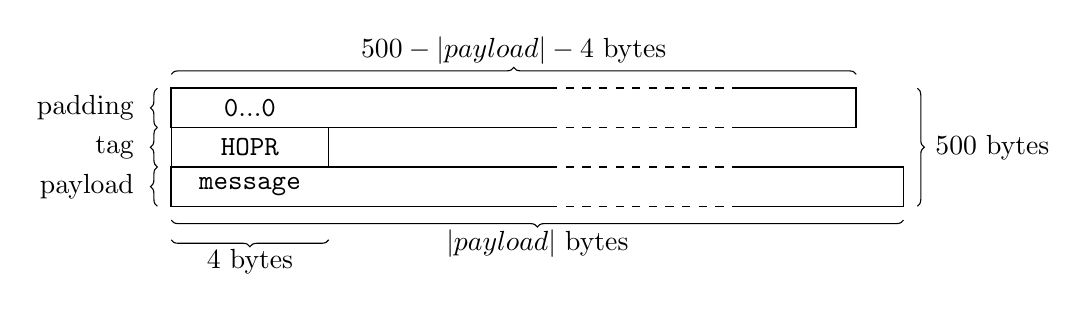
\begin{tikzpicture}
        \def\one{0.3}
        \def\lw{0.2}
        \def\middle{16*\one}
        \def\offset{8*\one}
        \def\packetLength{500}

        \def\paddingLength{29*\one}
        \def\payloadLength{31*\one}


        \draw[decoration={brace,raise=5pt},decorate] (0,0.5) -- node[above=5pt] {$\packetLength - |payload| - 4$ bytes} (\paddingLength,0.5);
        % \draw (0,-0.0) rectangle (\one*33,0.5);
        \begin{scope}
            \draw[decoration={brace,raise=5pt},decorate] (0,0) -- node[left=10pt] {padding} (0,0.5);
            \def\width{\paddingLength}
            \draw (1,0.25) node {$\mathtt{0...0}$};
            \draw [line width=\lw mm] (\middle,0.5) -- (0,0.5) --  (0,0) -- (\middle,0);
            \draw [line width=\lw mm] (\middle,0) --  (\middle+\offset, 0) [dashed];
            \draw [line width=\lw mm] (\middle,0.5) --  (\middle+\offset, 0.5) [dashed];
            \draw [line width=\lw mm] (\middle+\offset,0.5) -- (\width,0.5) --  (\width,0) -- (\middle+\offset,0);
        \end{scope}

        \begin{scope}[shift={(0,-0.5)}]
            \draw[decoration={brace,raise=5pt},decorate] (0,0) -- node[left=10pt] {tag} (0,0.5);
            \draw [draw] (0,0) rectangle (2,0.5);
            \draw (1,0.25) node {$\mathtt{HOPR}$};
        \end{scope}

        \begin{scope}[shift={(0,-1)}]
            \draw[decoration={brace,raise=5pt},decorate] (0,0) -- node[left=10pt] {payload} (0,0.5);
            \draw (1,0.25) node {$\mathtt{message}$};
            \def\width{\payloadLength}
            \draw [line width=\lw mm] (\middle,0.5) -- (0,0.5) --  (0,0) -- (\middle,0);
            \draw [line width=\lw mm] (\middle,0) --  (\middle+\offset, 0) [dashed];
            \draw [line width=\lw mm] (\middle,0.5) --  (\middle+\offset, 0.5) [dashed];
            \draw [line width=\lw mm] (\middle+\offset,0.5) -- (\width,0.5) --  (\width,0) -- (\middle+\offset,0);
        \end{scope}

        \draw[decoration={brace,raise=5pt,mirror},decorate] (0,-1.0) -- node[below=5pt] {$|payload|$ bytes} (\payloadLength,-1.0);
        \draw[decoration={brace,raise=5pt,mirror},decorate] (0,-1.25) -- node[below=5pt] {4 bytes} (2,-1.25);

        \draw[decoration={brace,raise=5pt},decorate] (\payloadLength,0.5) -- node[right=8pt] {$\packetLength$ bytes} (\payloadLength,-1.0);
    \end{tikzpicture}
    \caption{Padded message consisting of padding, tag $\tau$ ($\mathtt{0x484f5052}$, ASCII-encoded ``HOPR"), and payload $m$.}
\end{figure}

where $\tau$ is generated arbitrarily and $|\tau|=4$ is its length ($\tau=``HOPR "$ in ASCII). $l$ is the $0$ padding length where
$0 <= l <= |m| - 4$. The payloads that do not include the correct padding are considered invalid.

$m$ is divided into two blocks, left ($m_l$) and right ($m_r$), whose sizes are $|m_l|=w$ and $|m_r|=j-w$. We thus get $m=m_r\|m_l$.

\begin{comment}
\subparagraph{Encryption}
The blocks $m_l$ and $m_r$ are transformed using a four-round Feistel structure:

$$m_r\leftarrow m_r \oplus S_{u1}(m_l), m_l\leftarrow m_l \oplus H_{u2}(m_r), m_r\leftarrow m_r\oplus S_{u3}(m_l), m_l\leftarrow m_l\oplus H_{u4}(m_r)$$

The updated $m_l\|m_r$ constitutes the ciphertext $\delta$.
\end{comment}

\begin{comment}
\subparagraph{Decryption}
Decryption happens as follows:

$$m_l\leftarrow m_l\oplus H_{u4}(m_r), m_r\leftarrow S_{u3}(m_l), m_l\leftarrow m_l\oplus H_{u2}(m_r), m_r\leftarrow m_r\oplus S_{u1}(m_l)$$
\end{comment}